\documentclass{article}

\usepackage[margin=0.75in]{geometry}

\usepackage{polski}
\usepackage[utf8]{inputenc}

\usepackage{amsmath}
\usepackage{amssymb}
\usepackage{courier}
\usepackage{extpfeil}
\usepackage{float}
\usepackage{graphicx} % Required for inserting images
\usepackage{matlab-prettifier}
\usepackage{tcolorbox}


\usepackage[T1]{fontenc}
%\usepackage{tgbonum}

\title{
    Teoria Sterowania\\
    \Large Metody Częstotliwościowe
}
\author{Maciej Różewicz}
\date{2025}

\makeatletter         
\def\@maketitle{
\raggedright
\begin{center}
    
\includegraphics[width=0.5\linewidth]{fig/agh_logo.PNG}\\[8ex]
\end{center}
\begin{center}
    {\huge \bfseries \sffamily \@title }\\[4ex] 
    {\large  \@author}\\[4ex] 
    \@date\\[8ex]
\end{center}}
\makeatother

\begin{document}
\maketitle
\newpage

%%%%%%%%%%%%%%%%%%%%%%%%%%%%%%%%%%%%%%%%%%%%%%%%%%%%%%%%%%%%
\section{Cel ćwiczenia}
Celem ćwiczenia jest analiza stabilności systemów liniowych stacjonarnych za pomocą metod częstotliwościowych.
Będą to dwa kryteria:
\begin{itemize}
    \item kryterium Michajłowa - pozwala określić liczbę pierwiastków stabilnych i~niestabilnych równania charakterystycznego układu na podstawie znajomości jego współczynników,
    \item kryterium Nyquista - pozwala na określenie stabilności układu zamkniętego na podstawie znajomości charakterystyki częstotliwościowej układu otwartego (przy czym warto dodać, że kryterium to działa dla układów o~parametrach skupionych, jak i rozłożonych \cite{Gorecki1993} oraz dla układów z opóźnieniem) - dodatkowo kryterium Nyquista pozwala na określenie liczby pierwiastków w prawej półpłaszczyźnie układu zamkniętego.
\end{itemize}

%%%%%%%%%%%%%%%%%%%%%%%%%%%%%%%%%%%%%%%%%%%%%%%%%%%%%%%%%%%%
\section{Przebieg ćwiczenia}
\begin{enumerate}
    \item Rozważamy układ zamknięty z regulatorem proporcjonalnym $G_{R}(s) = K$, przedstawiony na rysunku (\ref{fig:zadanie_1}),
    gdzie transmitancja obiektu sterowanego wynosi:
    $$
        G_{0}(s) = \frac{s+1}{0.01s^{4} + 0.5s^{3} + 3s^{2} - 10s + 10}
    $$
    \begin{figure}[H]
        \centering
        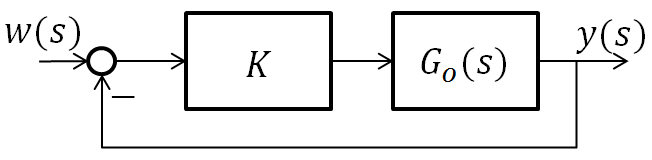
\includegraphics[width=0.75\linewidth]{fig/zadanie_1.png}
        \caption{Zamknięty układ regulacji.}
        \label{fig:zadanie_1}
    \end{figure}
    W czasie laboratorium:
    \begin{itemize}
        \item stosując kryterium Michajłowa wyznaczyć ilość niestabilnych biegunów transmitancji $G_{O}(s)$,
        \item stosując kryterium Nyquista określić wartości współczynnika $K \in \mathbb{R}_{+}$, dla których układ zamknięty będzie stabilny,
        \item wyrysować charakterystykę Bodego i Nicholsa, zaznaczyć zapas fazy i wzmocnienia.
    \end{itemize}
    
    \item Dany jest układ otwarty o transmitancji:
    $$
        G(s) = \frac{4}{s+1}e^{-0.5s}
    $$
    W czasie laboratorium:
    \begin{itemize}
        \item zbadać stabilność układu zamkniętego za pomocą kryterium Nyquista,
        \item sprawdzić, dla jakich wartości $K \in \mathbb{R}_{+}$ regulatora proporcjonalnego układ będzie stabilny,
        \item sprawdzić, dla jakiego opóźnienia układ przestanie być stabilny po zamknięciu pętli sprzężenia zwrotnego.
    \end{itemize}
\end{enumerate}


\end{document}
